\documentclass[10pt,a4paper]{article}
\usepackage{graphicx}
\usepackage[utf8]{inputenc}
\usepackage{amsmath}
\usepackage{amsfonts}
\usepackage{amssymb}
\author{TCP Solutions}
\title{Main project SRS}

\begin{document}

\begin{titlepage}
\begin{center}

\huge Software Requirements Specification\\[0.15cm]
\huge Forensic Medicine Mobile Application\\[0.15cm]
\large \texttt{Version: 1.0}\\[1cm]

Organization:\\
\texttt{University of Pretoria: TCP Solutions}\\[0.5cm]
GitHub:\\[0.01cm]

\begin{verbatim}
          https://github.com/CollenMphabantshi/TCP-Solutions
\end{verbatim}

Authors:\\
\texttt{Mr Mphambantshi C (10404687)\\
        Mr Legodi PT (29302732)\\
        Ms Sikhitha TP  (10404687)}\\[1cm]
        
May 22, 2014

\begin{tabular}{|l|l|l|}\hline
Name   & Date	& Changes	\\\hline
TP Solutions	& 14 May 2014	& Vision and Scope\\\hline
TP Solutions	& 15 May 2014	& Addition to vision and scope and quality requirements.\\\hline
TP Solutions	& 16 May 2014	& Software Architecture\\\hline
\end{tabular}

\end{center}
\end{titlepage}


\tableofcontents
\pagebreak
\section{Overview}
This document provides the overall vision and scope of the Forensic Medicine Mobile Application project. It explains and illustrates what the system will do and look like. This document basically provides the skeleton of our project. It includes the scope limitations and exclusions which will help guide the stakeholders on what is expected and not expected. This document also include use case diagram which will help explain and show the whole system.


\subsection{Document conventions}
\begin{description}
\item Documentation formulation: LaTeX
\item Unified Modelling Language: version 2.0
\end{description}

\section{Vision and Scope}

\begin{center}
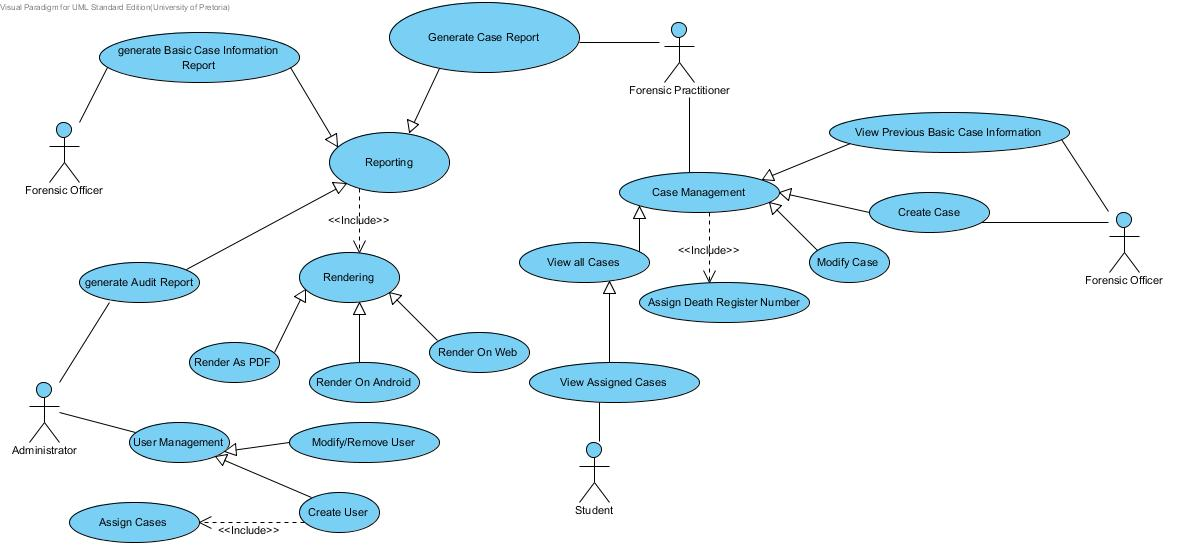
\includegraphics[scale=0.5]{DRUC.jpg}
\textbf{Figure 1: The Scope of the system}
\end{center}

The proposed system is the death scene register that allow:
 \begin{itemize}
 \item Forensic officers to: 
	 \begin{itemize}
		\item Capture data from death scene – the FO’s will gather information on every scene based on the template it has on the mobile application.
		\item View basic information. The FO views personal details of the deceased and police officer who was at the scene.
	\end{itemize}
\item Forensic practitioner to:
	 \begin{itemize}
		\item Generate reports – FP’s will generate web, android and pdf reports specifically to their needs e.g. generate report of all hanging cases 2014.
		\item View all cases – every scene stored on the database they should be able to view them.
		\item Edit case information. If there was any errors made on the form such as spelling errors FPs should be able to correct them.
		\item Manage cases. FPs will dictate if the case is natural and non-natural death and do other functionalities.
	 \end{itemize}
\item Students to:
	 \begin{itemize}
		\item View all the cases cleared to them – this is for research purpose only.
	 \end{itemize}
\item Administrator to:
	 \begin{itemize}
		\item Add new users.
		\item Remove users.
		\item Edit users – change personal details and access rights.
		\item View audit report.
	 \end{itemize}
\end{itemize}

\section{Scope Limitations and Exclusions}
Pictures that demonstrate how the incident happed are excluded on this phase, maybe they can be added at a later stage.

\pagebreak
\section{Architecture requirements}
\subsection{Access channel requirements}
\indent It is going to be accessed by humans using android and web application.
                                                                                               
\subsection{Quality requirements}
\begin{itemize}
\item\textbf{Performace}

               
\item\textbf{Reliability}
  
\item\textbf{Scalability}

 
\item\textbf{Security}

\item\textbf{Flexibility} 

\item\textbf{Maintanability}					
                         
\item\textbf{Auditability}         
          
\item\textbf{Usability}
                                                              
 \end{itemize}
\subsection{Integration requirements}
                
\subsection{Architecture constraint}                       

\pagebreak

\section{Functional Requirements}
\subsection{Introduction}


\subsection{Required functionality}




\subsection{Use case prioritization}


\subsection{Use case/Services contracts}

               
\pagebreak

\section{Open Issues}

\section{Glossary}
\begin{description}
	\item [Forensic officer (FO)] – a specially trained crime scene officer that collects the finding evidence that will be analyzed back at the lab by forensic scientist or forensic practitioner. 
	\item [Forensic practitioner (FP)] - also referred to as crime scene investigators and forensic science technicians examine pieces of evidence to provide crucial support in criminal investigations. Their professional expertise is sought in laboratories, crime scenes and courtrooms.
	\item [Stakeholders] - is anybody who can affect or is affected by an organization, strategy or project. They can be internal or external and they can be at senior or junior levels.
	\item [Students] – honors and masters students who are doing research as part of their studies.
	\item[MySQL] MySQL (Structured Query Language) is an open-source relational database management system.
	
	\item[PDF] Portable Document Format is a file format for capturing and sending electronic documents in exactly the intended format.
	\item[UML] Unified Modelling Language is a general-purpose modelling language in the field of software engineering. It provides a set of graphic notation techniques to create visual models of object-oriented software-intensive systems. 
	

\end{description}

\end{document}
